\documentclass[10pt,landscape]{article}
\usepackage{amssymb,amsmath,amsthm,amsfonts}
\usepackage{multicol,multirow}
\usepackage{calc}
\usepackage{ifthen}
\usepackage[landscape]{geometry}
\usepackage[colorlinks=true,citecolor=blue,linkcolor=blue]{hyperref}
\usepackage{graphicx}
\usepackage{subcaption}


\ifthenelse{\lengthtest { \paperwidth = 11in}}
    { \geometry{top=.2in,left=.2in,right=.2in,bottom=.2in} }
	{\ifthenelse{ \lengthtest{ \paperwidth = 297mm}}
		{\geometry{top=1cm,left=1cm,right=1cm,bottom=1cm} }
		{\geometry{top=1cm,left=1cm,right=1cm,bottom=1cm} }
	}
\pagestyle{empty}
\makeatletter
\renewcommand{\section}{\@startsection{section}{1}{0mm}%
                                {-1ex plus -.5ex minus -.2ex}%
                                {0.5ex plus .2ex}%x
                                {\normalfont\large\bfseries}}
\renewcommand{\subsection}{\@startsection{subsection}{2}{0mm}%
                                {-1explus -.5ex minus -.2ex}%
                                {0.5ex plus .2ex}%
                                {\normalfont\normalsize\bfseries}}
\renewcommand{\subsubsection}{\@startsection{subsubsection}{3}{0mm}%
                                {-1ex plus -.5ex minus -.2ex}%
                                {1ex plus .2ex}%
                                {\normalfont\small\bfseries}}
                            
\newcommand{\de}{\mathrm d}
\newcommand{\fracd}[2]{\frac{\de #1}{\de #2}}
\newcommand{\fracp}[2]{\frac{\partial #1}{\partial #2}}
\newcommand{\fracpq}[2]{\frac{\partial^2 #1}{{\partial #2}^2}}
\newcommand{\fracpp}[3]{\frac{\partial^2 #1}{\partial #2 \partial #3}}
\newcommand{\dive}[1]{\text{div}\,#1}
\newcommand{\rot}[1]{\text{rot}\,#1}
\newcommand{\sz}[1]{\scriptsize #1\normalsize}
\newcommand{\ul}[1]{\underline{\smash{#1}}}
\newcommand{\mach}{\text{Ma}}
\makeatother
\setcounter{secnumdepth}{0}
\setlength{\parindent}{0pt}
\setlength{\parskip}{0pt plus 0.5ex}
% -----------------------------------------------------------------------
\begin{document}

\raggedright
\footnotesize

\begin{center}
\Large\textbf{COORDINATE CURVILINEE}
\end{center}
\begin{multicols*}{2}
\setlength{\premulticols}{1pt}
\setlength{\postmulticols}{1pt}
\setlength{\multicolsep}{1pt}
\setlength{\columnsep}{2pt}

\section{Generalità}
$\Omega',\Omega \subset \mathbb{R}^N\quad \Phi:\Omega' \rightarrow \Omega$ diffeomorfismo $\quad u\in \Omega' \quad x=\Phi(u)\in \Omega$\\

$(u,v,w)$ è destrorso $\Longleftrightarrow \det(J\Phi)=\det \left(\fracp{(x_1,x_2,x_3)}{(u_1,u_2,u_3)}\right)>0$\\

\subparagraph{linee coordinate} $\Gamma_i=\{x\in \Omega\;|\;x=\Phi(\bar u+t\mathbf u_i,t\in\mathbb{R}\}$\\
\subparagraph{superfici coordinate} $\Sigma_i=\{\}$\\\;

Da qui in poi $N=3\;\;$ e $\begin{array}{l}\Phi(u_1,u_2,u_3)=(X_1(u_1,u_2,u_3),X_2(u_1,u_2,u_3),X_3(u_1,u_2,u_3))\\ \Phi^{-1}(x_1,x_2,x_3)=(U_1(x_1,x_2,x_3),U_2(x_1,x_2,x_3),U_3(x_1,x_2,x_3))\end{array}$\\

\subparagraph{trasformazione diretta}$\quad (u_1,u_2,u_3)\overset{\Phi}{\mapsto}(x_1,x_2,x_3)$\\
\subparagraph{trasformazione inversa}$\quad (x_1,x_2,x_3)\overset{\Phi^{-1}}{\mapsto}(u_1,u_2,u_3)$\\\;

\subparagraph{fattori di scala e versori}\mbox{}\\
$\mathbf r =x_1\,\mathbf i+x_2\,\mathbf j+x_3\,\mathbf k=u_1\mathbf u_1+u_2\mathbf u_2+u_3\mathbf u_3
\quad h_i=\|\frac{\partial \mathbf r}{\partial u_i}\|%=\sqrt{(\fracp{X_1}{u_1})^2+(\fracp{X_2}{u_1})^2+(\fracp{X_3{u_1})^2}
\qquad\mathbf u_i=\frac 1{h_i}\fracp{\mathbf r}{u_i}$\\\;

\subparagraph{elementi infinitesimi}\mbox{}\\
%lunghezze%
$\begin{array}{l}
\mathrm{d}\mathbf r=h_1\mathrm{d}u_1\mathbf u_1+h_2\mathrm{d}u_2\mathbf u_2+h_3\mathrm{d}u_3\mathbf u_3\\
\mathrm{d}s^2={h_1}^2{\mathrm{d}u_1}^2+{h_2}^2{\mathrm{d}u_2}^2+{h_3}^2{\mathrm{d}u_3}^2\end{array}\qquad
%aree e volume%
\begin{array}
{l}\mathrm{d}S_1=h_2h_3\mathrm{d}u_2\mathrm{d}u_3\\
\mathrm{d}S_2=h_1h_3\mathrm{d}u_1\mathrm{d}u_3\\
\mathrm{d}S_3=h_1h_2\mathrm{d}u_1\mathrm{d}u_2
\end{array}\qquad
\mathrm{d}V=h_1h_2h_3\mathrm{d}u_1\mathrm{d}u_2\mathrm{d}u_3$\\\;

\subparagraph{componenti di un campo vettoriale}\mbox{}\\
$\;\,F_{u_i}={h_i}\left(F_{x_1}\fracp{X_1}{u_1}+F_{x_2}\fracp{X_2}{u_1}+F_{x_3}\fracp{X_3}{u_1}\right)$\\\;\;

\subparagraph{operatori differenziali}\mbox{}\\
$\;\,\nabla f=\sum\frac1{h_i}\fracp{f}{u_i}\mathbf u_i\qquad\qquad
\nabla \cdot \mathbf F=\frac1{h_1h_2h_3}\sum\frac{\partial}{\partial u_i}\left(\frac{h_1h_2h_3}{h_i}F_{u_i}\right)$\\
$\;\,\nabla\times\mathbf F=\frac1{h_1h_2h_3}\det\left(\begin{matrix}
h_1\mathbf u_1&h_2\mathbf u_2&h_3\mathbf u_3\\
\fracp{}{u_1}&\fracp{}{u_2}&\fracp{}{u_3}\\
h_1F_{u_1}&h_2F_{u_2}&h_3F_{u_3}\end{matrix}\right)\qquad\qquad
\nabla^2 f=\frac1{h_1h_2h_3}\sum\fracp{}{u_i}\left(\frac{h_1h_2h_3}{h_i}\fracp{f}{u_i}\right)$\\

%cambi notevoli
\section{Cambi notevoli di coordinate}

\subsection{coordinate cilindriche\textbackslash polari}
$\Phi_C:\mathbb{R}_0^+\times [0,2\pi)\times\mathbb{R}\rightarrow\mathbb{R}^3\qquad
\begin{array}{l}(\rho,\theta,z)\overset{\Phi_C}{\mapsto}(\rho\cos\theta,\rho\sin\theta,z)\\
(x_1,x_2,x_3)\overset{\Phi_C^{-1}}{\mapsto}(\sqrt{x_1^2+x_2^2},\arctan_2(x_2/x_1),x_3)\end{array}$\\

$\det(J\Phi_C)=\det\left(\begin{matrix}\cos\theta&-\rho\sin\theta&0\\ \sin\theta&\rho\cos\theta&0\\0&0&1\end{matrix}\right)=\rho>0\qquad
\begin{array}{l}h_\rho=1\\h_\theta=\rho\\h_z=1\end{array}\qquad
\begin{array}{l}\hat u_\rho=\cos\theta\,\mathbf i+\sin\theta\,\mathbf j\\\hat u_\theta=-\sin\theta\,\mathbf i+\cos\theta\,\mathbf j\\ \hat u_z=\mathbf k\end{array}$\\

$\begin{array}{l}\mathrm{d}\mathbf r=\mathrm{d}\rho\,\hat u_\rho+\rho\,\mathrm{d}\theta\,\hat u_\theta+\mathrm{d}z\,\hat u_z\\
\mathrm{d}s^2=\mathrm{d}\rho^2+\rho^2\mathrm{d}\theta^2+\mathrm{d}z^2\end{array}\qquad
\begin{array}{l}\mathrm{d}S_\rho=\rho\,\mathrm{d}\theta\,\mathrm{d}z\\\mathrm{d}S_\theta=\mathrm{d}\rho\,\mathrm{d}z\\\mathrm{d}S_z=\rho\,\mathrm{d}\rho\,\mathrm{d}\theta\end{array}\qquad
\mathrm{d}V=\rho\,\mathrm{d}\rho\,\mathrm{d}\theta\,\mathrm{d}z$

$\nabla f=\fracp{f}{\rho}\mathbf u_\rho + \frac1\rho\fracp{f}{\theta}\mathbf u_\theta+\fracp{f}{z}\mathbf u_z$\\
$\nabla\cdot\mathbf F=\fracp{f}{\rho}\mathbf + \frac1\rho\fracp{f}{\theta} +\fracp{f}{z}$\\
$

\subsection{coordinate sferiche}
$\Phi_S:\mathbb{R}_0^+\times[0,\pi]\times [0,2\pi)\rightarrow\mathbb{R}^3\qquad
\begin{array}{l}(r,\varphi,\theta)\overset{\Phi_S}{\mapsto}(r\sin\varphi\cos\theta,r\sin\varphi\sin\theta,r\cos\varphi)\\
(x,y,z)\overset{\Phi_S^{-1}}{\mapsto}()\end{array}$\\

$J\Phi_S=\left(\begin{matrix}\sin\varphi\cos\theta&r\cos\varphi\cos\theta&-r\sin\varphi\sin\theta\\\sin\varphi\sin\theta&r\cos\varphi\sin\theta&r\sin\varphi\cos\theta\\\cos\varphi&-r\sin\varphi&0\end{matrix}\right)\qquad\det(J\Phi_S)=r\sin^2\varphi>0$\\
$\begin{array}{l}h_r=1\\h_\varphi=r\\h_\theta=r\sin\varphi\end{array}\qquad
\begin{array}{l}\hat u_r=\sin\varphi\cos\theta\,\mathbf i+\sin\varphi\sin\theta\,\mathbf i+\cos\varphi\,\mathbf k\\\hat u_\varphi=\cos\varphi\cos\theta\,\mathbf i+\cos\varphi\sin\theta\,\mathbf i-\sin\varphi\,\mathbf k\\\hat u_\theta=-\sin\theta\,\mathbf i+\cos\theta\,\mathbf j\end{array}$\\
$\begin{array}{l}\mathrm{d}\mathbf r=\mathrm{d}r\,\hat u_r+r\,\mathrm{d}\varphi\,\hat u_\varphi+r\sin\varphi\,\mathrm{d}\theta\,\hat u_\theta\\
\mathrm{d}s^2=\mathrm{d}\rho^2+r^2\mathrm{d}\varphi^2+r^2\sin^2\varphi\,\mathrm{d}\theta^2\end{array}\qquad
\begin{array}{l}\mathrm{d}S_r=r^2\sin\varphi\,\mathrm{d}\varphi\,\mathrm{d}\theta\\\mathrm{d}S_\varphi=r\sin\varphi\,\mathrm{d}r\,\mathrm{d}\theta\\\mathrm{d}S_\theta=r\,\mathrm{d}r\,\mathrm{d}\varphi\end{array}\qquad
\mathrm{d}V=r^2\sin\varphi\,\mathrm{d}r\,\mathrm{d}\varphi\,\mathrm{d}\theta$
\vfill\null\columnbreak

\subsection{riflessioni assi}
$\Phi_X:\mathbb{R}^2\longrightarrow\mathbb{R}^2\qquad
\begin{array}{l}(\xi,\eta)\overset{\Phi_X}{\mapsto}(\xi,-\eta)\\(x,y)\overset{\Phi_X^{-1}}{\mapsto}(x,-y)\end{array}\qquad
\det(J\Phi_X)=\det=\left(\begin{matrix}1&0\\0&-1\end{matrix}\right)=-1<0$\\
$\begin{array}{l}h_\xi=1\\h_\eta=1\end{array}\qquad
\begin{array}{l}\hat u_\xi=\mathbf i\\\hat u_\eta=-\mathbf j\end{array}\qquad
\begin{array}{l}\mathrm{d}\mathbf r=\mathrm{d}\xi\,\mathbf i-\mathrm{d}\eta\,\mathbf j\\\mathrm{d}s^2=\mathrm{d}\xi^2+\mathrm{d}\eta^2\end{array}\qquad
\mathrm{d}S=\mathrm{d}\xi\,\mathrm{d}\eta$\\\qquad

$\Phi_Y:\mathbb{R}^2\longrightarrow\mathbb{R}^2\qquad
\begin{array}{l}(\xi,\eta)\overset{\Phi_Y}{\mapsto}(-\xi,\eta)\\(x,y)\overset{\Phi_Y^{-1}}{\mapsto}(-x,y)\end{array}\qquad
\det(J\Phi_Y)=\det=\left(\begin{matrix}-1&0\\0&1\end{matrix}\right)=-1<0$\\
$\begin{array}{l}h_\xi=1\\h_\eta=1\end{array}\qquad
\begin{array}{l}\hat u_\xi=-\mathbf i\\\hat u_\eta=\mathbf j\end{array}\qquad
\begin{array}{l}\mathrm{d}\mathbf r=-\mathrm{d}\xi\,\mathbf i+\mathrm{d}\eta\,\mathbf j\\\mathrm{d}s^2=\mathrm{d}\xi^2+\mathrm{d}\eta^2\end{array}\qquad
\mathrm{d}S=\mathrm{d}\xi\,\mathrm{d}\eta$\\
\;\;\;\;\;\;\;\;\;
\begin{tabular}{c c}
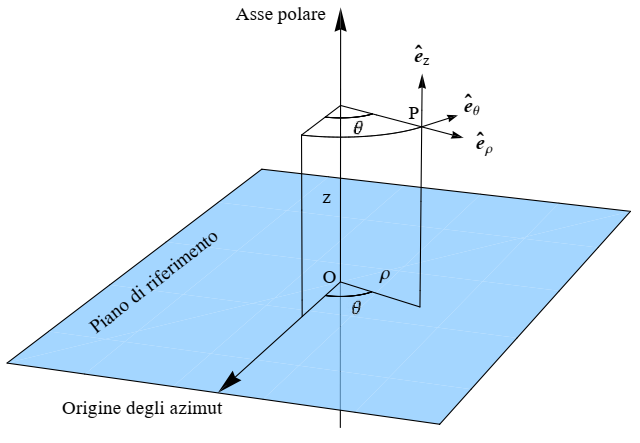
\includegraphics[width=4cm]{cyl}&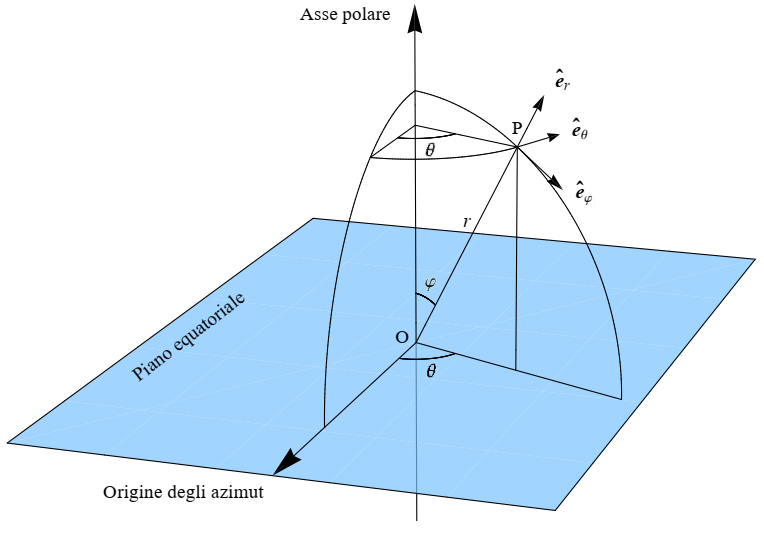
\includegraphics[width=4cm]{sph}\\
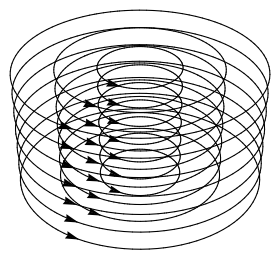
\includegraphics[width=4cm]{c1cyl}&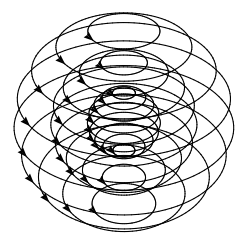
\includegraphics[width=4cm]{c1sph}\\
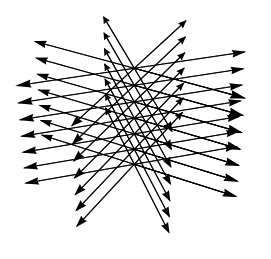
\includegraphics[width=4cm]{c2cyl}&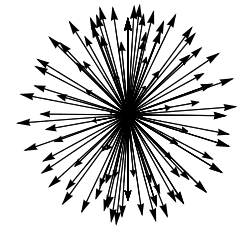
\includegraphics[width=4cm]{c2sph}\\
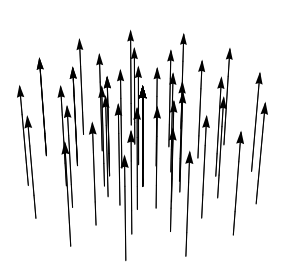
\includegraphics[width=4cm]{c3cyl}&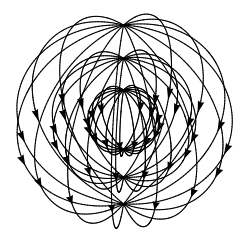
\includegraphics[width=4cm]{c3sph}
\end{tabular}
\vfill\null\columnbreak
sistema cilindrico\\sistema sferico\\
$\rho$ costante\\$r$ costante\\
$\theta$ costante\\$\varphi$ costante\\
$z$ costante\\$\theta$ costante



\end{multicols*}
\end{document}
